\documentclass[11pt,letterpaper]{article}
\usepackage[margin=0.72in]{geometry}
\usepackage[T1]{fontenc}
\usepackage{lmodern,microtype,booktabs,graphicx,xcolor,array}
\usepackage[colorlinks=true,urlcolor=blue,linkcolor=blue]{hyperref}
\definecolor{ink}{HTML}{172B36}
\definecolor{light}{HTML}{EEF4F7}
\color{ink}
\setlength{\parindent}{0pt}
\setlength{\parskip}{6pt}
\setlength{\tabcolsep}{6pt}
\renewcommand{\arraystretch}{1.12}
\hypersetup{pdftitle={Current disaster funding exports do not establish past county totals},pdfauthor={James N. Jean}}
\newcommand{\CurrentRecords}{17,994}
\newcommand{\SourceGroups}{132}
\newcommand{\SufficientCells}{9,844}
\newcommand{\ProbeCount}{1,340}
\newcommand{\CurrentGroups}{134}
\newcommand{\MetaCaptures}{2}
\newcommand{\ValueCaptures}{1}
\newcommand{\PastCaptures}{0}
\newcommand{\NativeChecks}{141,166}
\newcommand{\SavedChecks}{49,237}
\newcommand{\ProbeChecks}{18,526}
\newcommand{\FixtureCount}{38}
\newcommand{\FreezeCount}{26}
\newcommand{\FigureChecks}{910}
\newcommand{\FigureBars}{44}
\newcommand{\SvgCoordinates}{176}
\newcommand{\PythonOld}{3.10.11}
\newcommand{\PythonNew}{3.12.14}
\newcommand{\ReplaySources}{11}
\newcommand{\ThreeCodes}{68}
\newcommand{\OtherCodes}{64}
\newcommand{\MixedGroups}{22}
\newcommand{\OtherLabels}{110}
\newcommand{\LabelsAustin}{Austin County; Statewide}
\newcommand{\LabelsDallas}{Dallas County; Statewide}
\newcommand{\LabelsHarris}{Harris County; Statewide}
\newcommand{\RecordsA}{6,621}
\newcommand{\CurrentMoneyA}{2,999,825,482.86}
\newcommand{\CutoffA}{2018-12-31}
\newcommand{\FirstCountAA}{3,155}
\newcommand{\StoreCountAA}{0}
\newcommand{\FirstMoneyA}{1,372,714,981.32}
\newcommand{\FirstRecordPercentA}{47.65}
\newcommand{\FirstDollarPercentA}{45.76}
\newcommand{\CutoffB}{2020-12-31}
\newcommand{\FirstCountAB}{6,254}
\newcommand{\StoreCountAB}{0}
\newcommand{\CutoffC}{2022-12-31}
\newcommand{\FirstCountAC}{6,582}
\newcommand{\StoreCountAC}{0}
\newcommand{\CutoffD}{2024-12-31}
\newcommand{\FirstCountAD}{6,601}
\newcommand{\StoreCountAD}{0}
\newcommand{\CutoffE}{2026-10-30}
\newcommand{\FirstCountAE}{6,621}
\newcommand{\StoreCountAE}{6,621}
\newcommand{\RecordsB}{11,373}
\newcommand{\CurrentMoneyB}{35,573,517,223.51}
\newcommand{\FirstCountBA}{875}
\newcommand{\StoreCountBA}{0}
\newcommand{\FirstMoneyB}{5,993,968,800.80}
\newcommand{\FirstRecordPercentB}{7.69}
\newcommand{\FirstDollarPercentB}{16.85}
\newcommand{\FirstCountBB}{6,329}
\newcommand{\StoreCountBB}{0}
\newcommand{\FirstCountBC}{10,350}
\newcommand{\StoreCountBC}{0}
\newcommand{\FirstCountBD}{11,142}
\newcommand{\StoreCountBD}{0}
\newcommand{\FirstCountBE}{11,373}
\newcommand{\StoreCountBE}{11,373}
\begin{document}
{\Large\bfseries Current disaster funding exports do not establish past county totals\par}
{\large An OpenFEMA snapshot-availability audit and implementation exercise\par}
James N. Jean \hfill Independent research, 30 October 2026\\
{\small Source capture: 31 October 2026 UTC. Not peer reviewed. No FEMA endorsement.}

\section*{The practical decision}
A county dashboard needs actual dated financial values and the right geographic meaning. Filtering today's records by a date field supplies neither automatically.

This fixed audit captures \CurrentRecords{} current records for disasters 4332 and 4339. A \texttt{lastRefresh} filter selects none at the four pre-2026 probes, while a first-obligation-date filter retains different portions of today's records. Those zeroes do not establish zero historical funding. In addition, \MixedGroups{} raw source county-code groups mix a named county with Statewide labels; they cannot be allocated to physical counties without further evidence.

\colorbox{light}{\parbox{\dimexpr\linewidth-2\fboxsep\relax}{\textbf{Recommended action.} Archive the actual county-value tables with their source and population definitions. Reject metadata-only captures and current-record filters as historical values. Resolve geographic mappings before comparing counties.}}

\small
\begin{tabular}{@{}lrr@{}}
\toprule
Fixed cohort & Current records & Current reported federal field (USD)\\
\midrule
4332, TX & \RecordsA{} & \CurrentMoneyA{}\\
4339, PR & \RecordsB{} & \CurrentMoneyB{}\\
\bottomrule
\end{tabular}
\normalsize

{\small\textbf{Table 1.} The field is \texttt{federalShareObligated}: reported grant funding available to the grantee, not paid cash, official financial reporting or funding observed at an earlier date. All records meet the prespecified monetary identity/finite-value criteria in this capture.}

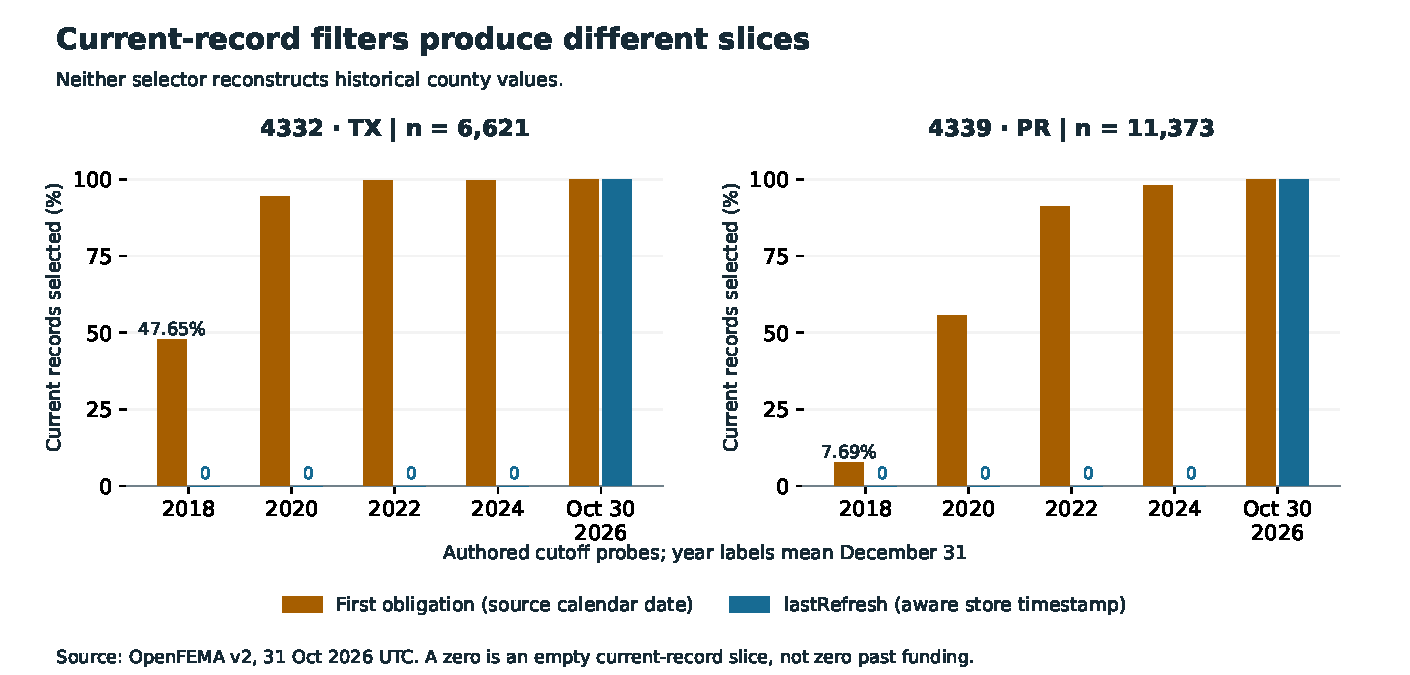
\includegraphics[width=\linewidth]{images/current_record_probes.pdf}
{\small\textbf{Figure 1.} Selected fractions of the current record denominator in each cohort. First obligation uses the source calendar day; store update requires an aware UTC timestamp. Neither selector reconstructs historical county values.}
\newpage

\section*{Two selectors, two slices of the current capture}
The first probe is 31 December 2018. For 4332, the source first-obligation calendar filter selects \FirstCountAA{} current records (\FirstRecordPercentA{}\%) carrying \FirstMoneyA{} current reported dollars. For 4339, it selects \FirstCountBA{} records (\FirstRecordPercentB{}\%) carrying \FirstMoneyB{} current reported dollars. These amounts may have changed after the first obligation date. They are not estimates of the amounts visible in 2018.

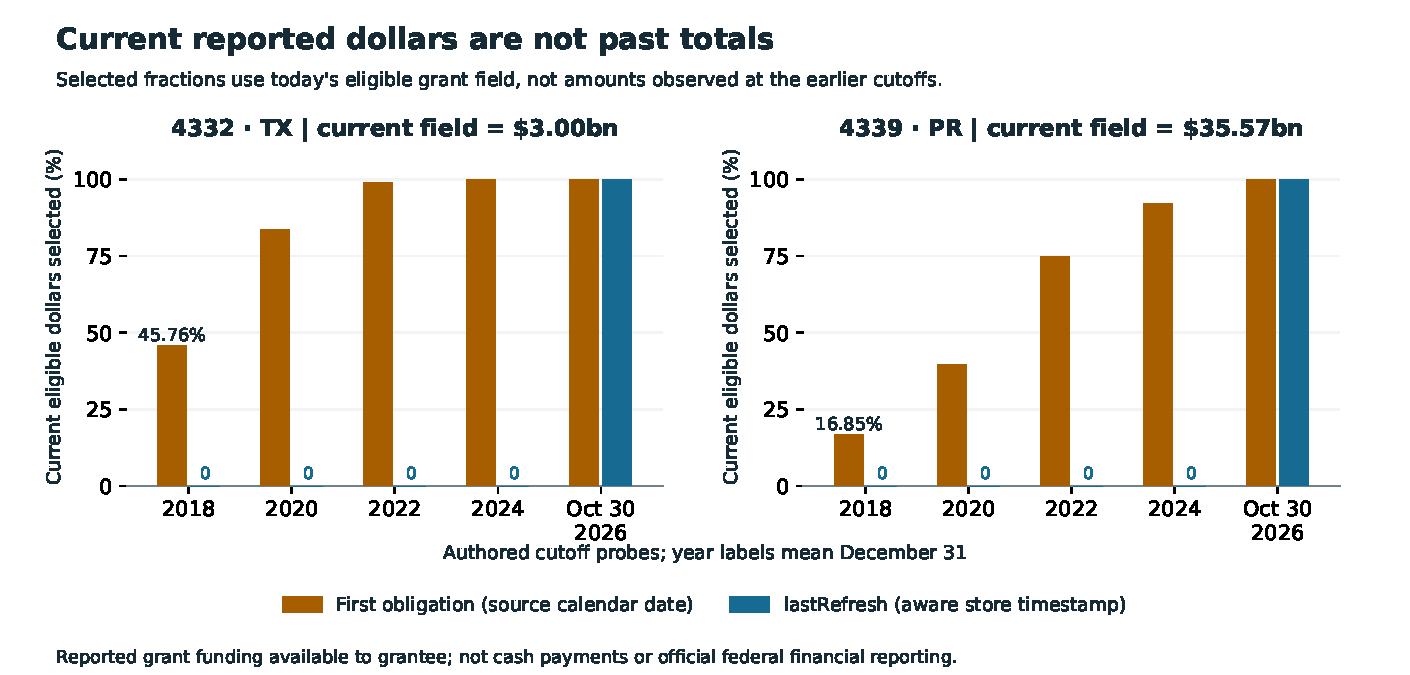
\includegraphics[width=\linewidth]{images/current_dollar_probes.pdf}
{\small\textbf{Figure 2.} Selected fractions of the current eligible monetary field. The earliest first-obligation slices contain \FirstDollarPercentA{}\% and \FirstDollarPercentB{}\% of today's respective denominators. A store-refresh date is not an original publication time. A zero selected sum describes an empty current-record slice, not zero past funding.}

\small
\begin{tabular}{@{}llrr@{}}
\toprule
Disaster & Authored cutoff & First-obligation records & Store-refresh records\\
\midrule
4332 & \CutoffA & \FirstCountAA & \StoreCountAA \\
4332 & \CutoffB & \FirstCountAB & \StoreCountAB \\
4332 & \CutoffC & \FirstCountAC & \StoreCountAC \\
4332 & \CutoffD & \FirstCountAD & \StoreCountAD \\
4332 & \CutoffE & \FirstCountAE & \StoreCountAE \\
4339 & \CutoffA & \FirstCountBA & \StoreCountBA \\
4339 & \CutoffB & \FirstCountBB & \StoreCountBB \\
4339 & \CutoffC & \FirstCountBC & \StoreCountBC \\
4339 & \CutoffD & \FirstCountBD & \StoreCountBD \\
4339 & \CutoffE & \FirstCountBE & \StoreCountBE \\
\bottomrule
\end{tabular}
\normalsize

{\small\textbf{Table 2.} Both selectors at every fixed disaster-level probe. Counts refer to current records. The complete \ProbeCount{} county-group and disaster-level cases retain exact current-dollar sums, fractions, unknown-date counts and denominators in the CSV exports. Year-end cutoffs are 23:59:59 UTC; first obligation is compared at source calendar-day resolution.}

The late 2026 probe selects all current records under both filters. That agreement does not establish historical stability or original publication availability.
\newpage

\section*{County codes do not establish where work occurred}
FEMA defines county as the applicant location. It can differ from the location of damaged work. The current source projection contains \SourceGroups{} raw county-code/name groups, not \SourceGroups{} verified physical counties or county spending estimates.

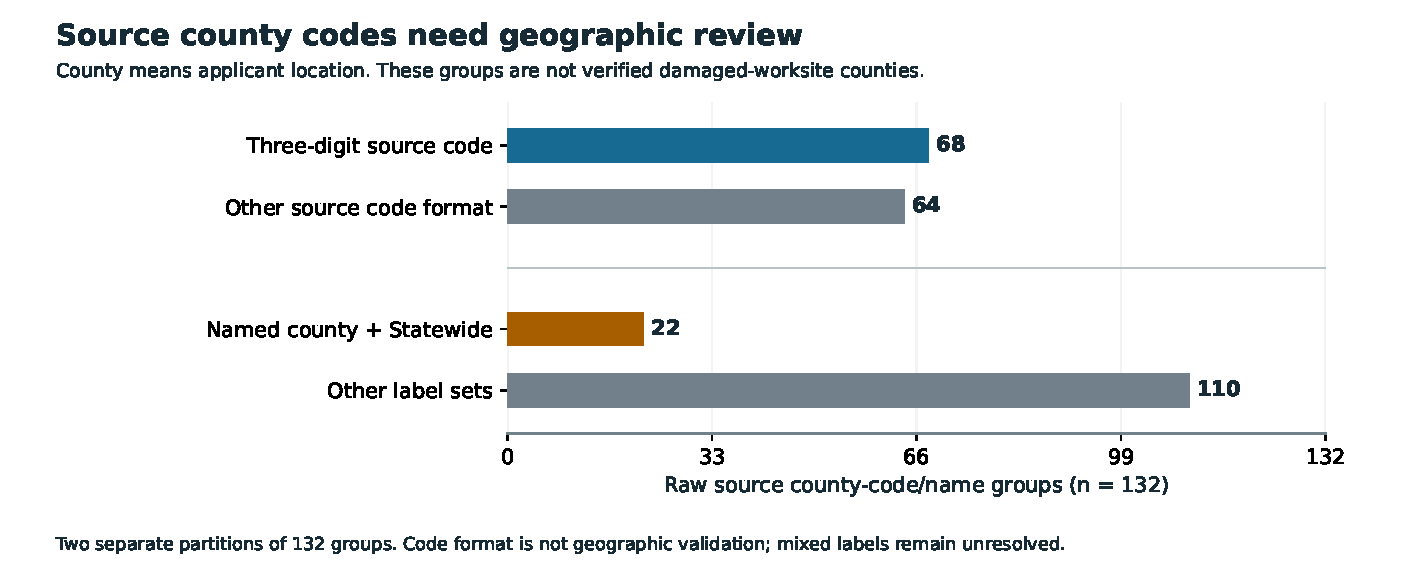
\includegraphics[width=\linewidth]{images/source_county_flags.pdf}
{\small\textbf{Figure 3.} Two separate partitions of the same \SourceGroups{} source groups: \ThreeCodes{} have three-digit source codes and \OtherCodes{} have another format; \MixedGroups{} mix Statewide and named county labels, while \OtherLabels{} have other label sets. Code format alone does not establish correct or incorrect geography.}

Examples from the TX cohort retain the exact source labels:

\small
\begin{tabular}{@{}ll@{}}
\toprule
Raw county code & Retained source county names\\
\midrule
15 & \LabelsAustin{}\\
113 & \LabelsDallas{}\\
201 & \LabelsHarris{}\\
\bottomrule
\end{tabular}
\normalsize

A short numeric code may need formatting review; it is not declared invalid. A group containing Statewide and a named county remains unresolved for geographic allocation. No dollars are assigned to a damaged-worksite county or ranked as local funding need.

\section*{Metadata is a different kind of evidence}
The packet contains \MetaCaptures{} actual metadata observations and \ValueCaptures{} current county-value capture. It establishes \PastCaptures{} earlier county-value tables. Nine inspected metadata fields agree between the two observations, including the reported global record count, metadata-update time and dataset-reload time. The captured response hashes differ.

Equal metadata does not supply previous monetary values. The metadata record's \texttt{lastRefresh}, the dataset's \texttt{lastDataSetRefresh} and a funded record's \texttt{lastRefresh} have distinct meanings. A completed reload does not prove that individual records changed or stayed unchanged. The original stability-horizon question remains unexecuted.
\newpage

\section*{Methods and the local comparison guard}
The two disaster numbers and five calendar probes were fixed before project retrieval. Metadata and definitions were already visible, so selection is source informed, not blinded. The scope is the original protocol's data-availability alternative, rather than a reconstructed historical revision curve.

All matching API pages, counts, exact request parameters and payload hashes are retained. Final declared counts and the dataset-refresh marker agree across capture, which does not prove atomicity. Native project records remain private. Public data contain \SufficientCells{} county/date sufficient cells and complete source names, eligibility and unknown-state accounting.

The monetary field is never combined with project cost or overlapping obligation measures. Exact source decimals are accumulated at an authored 80-digit working precision and independently checked as rational values. Missing amounts never become zero; negative adjustments would retain their sign. This capture has no missing/duplicate project identity, missing monetary amount or unknown studied date. Calendar probes and display precision are authored settings, not tuned deadlines or learned parameters.

The seven source-backed requests produce:

\small
\begin{tabular}{@{}p{0.47\linewidth}p{0.47\linewidth}@{}}
\toprule
Request & Outcome\\
\midrule
Qualified current county-group description & Accept with source qualifications\\
Two metadata captures as financial history & Reject missing actual county values\\
Current store-date filter as financial history & Reject missing actual county values\\
Applicant county as damaged-worksite county & Reject definition mismatch\\
Grant field as paid cash & Reject definition mismatch\\
Absent evidence identifier & Reject missing evidence\\
A historical stability horizon & Reject unestablished horizon\\
\bottomrule
\end{tabular}
\normalsize

The guard checks curated definition tags, evidence kind, coverage, hashes and time order. It does not independently certify geographic mappings or another producer's assertions. A two-value comparison accepted in an authored fixture demonstrates the interface only; it is not an observed historical comparison in this packet. No deployment or measured workflow saving is claimed.

\textbf{Independent checks.} \FreezeCount{} source/method dependencies were committed before cutoff comparisons. Strict native JSON tokens, a separate date parser, SQLite group/key reconstruction and exact Fraction sums pass \NativeChecks{} finite conditions. Saved-source checks pass \SavedChecks{}. Every \CurrentGroups{} current group and \ProbeCount{} probe is independently reconstructed through \ProbeChecks{} exact-rational/calendar conditions. The \FixtureCount{} authored tests cover provenance, date ambiguity, signed values, missingness, duplicate identity paths and empty denominators. These are finite checks, not universal correctness.
\newpage

\section*{Reproduce the fixed audit}
Two separate full-history checkouts, CPython \PythonOld{} and \PythonNew{}, reproduce all five analysis/exercise result files byte for byte, with \ReplaySources{} data-directory files unchanged in each. This saved-data replay does not redownload mutable native sources or repeat native source acquisition.

\begin{verbatim}
python -m pip install -r requirements.txt
python src/replay.py --out ../disaster-audit-replay
\end{verbatim}

The package contains the fixed protocol, source definitions, complete source exclusions and case exports, the guard, fixtures, independent source/result checkers and three original figures. Figure verification checks \FigureBars{} actual source-bound bars, \SvgCoordinates{} SVG coordinate conditions, numeric labels and nine hashes through \FigureChecks{} finite conditions. Native reacquisition must be treated as a new mutable-source capture, not silently substituted into this fixed version.

\section*{Limits and evidence still needed}
This is a finite convenience cohort of two declarations, not a national sample or a funding-need analysis. Public Assistance funded-project records exclude pre-obligation projects, and system migration can change the reporting population. The financial field comes from Grants Manager rather than FEMA's official financial systems and is not intended for official federal reporting.

The current record's first obligation date does not recover an earlier amount. A store refresh time does not establish source-system change time or original availability. Metadata observations do not establish county financial history. The stability horizon, true historical revision error and waiting period remain unknown. County-code/name groups are not certified geographic units.

A follow-up needs repeated actual county-value snapshots, a consistent population and documented geographic reconciliation. The local guard can check declared evidence types; it cannot create missing history or prove another producer's assertions. There is no causal recovery effect, financial saving, national reliability estimate, predictive improvement or new-estimator claim.

\section*{Primary sources, attribution and publication}
{\small
FEMA, \href{https://www.fema.gov/api/open/v2/PublicAssistanceFundedProjectsDetails}{PublicAssistanceFundedProjectsDetails v2};
\href{https://www.fema.gov/openfema-data-page/public-assistance-funded-projects-details-v2}{field dictionary};
\href{https://www.fema.gov/about/openfema/api}{API definitions};
\href{https://www.fema.gov/about/openfema/terms-conditions}{Terms and Conditions}.
Native project capture: 31 October 2026 UTC; exact request times, URLs and hashes are retained. Statistical research/reporting only: no individual-assistance records, reidentification, benefit-eligibility decisions, agency seals or endorsement.

This product uses the Federal Emergency Management Agency's OpenFEMA API, but is not endorsed by FEMA. The Federal Government or FEMA cannot vouch for the data or analyses derived from these data after the data have been retrieved from the Agency's website(s).

This is an independent program manuscript, not a formal-publication submission. Azure optimization and other formal-publication projects remain private.
}
\end{document}
